\subsection{PIMS Artificial Intelligence Module}
This module is responsible for predicting the chances of survival for each cancer type. Parameters for each patient are considered to compute this prediction. These parameters are converted into a single value that will be used by the PIMS Neural Network Module as input. \par 

\subsubsection{Scope}
The scope is shown in the use case diagram below: \par
\begin{figure}[H]
\centerline{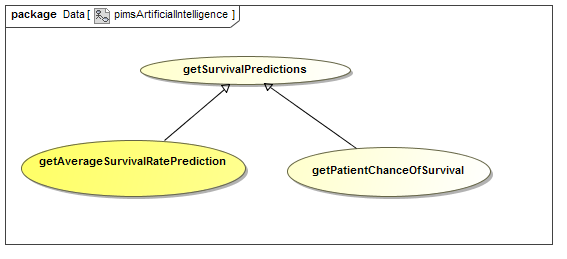
\includegraphics[width=0.75\linewidth]{./Functional_Requirements/Graphics/pimsAI/pimsArtificialIntelligence}}
\caption{The global scope for PIMS Artificial Intelligence Module}
\end{figure}

\subsubsection{Use cases}
\begin{description}

	\item{\textbf{getAverageSurvivalRatePrediction -- [priority: critical]}}
	\begin{description}
		\item{\textbf{Service Contract}} The generic service contract
		\begin{figure}[H]
			\centerline{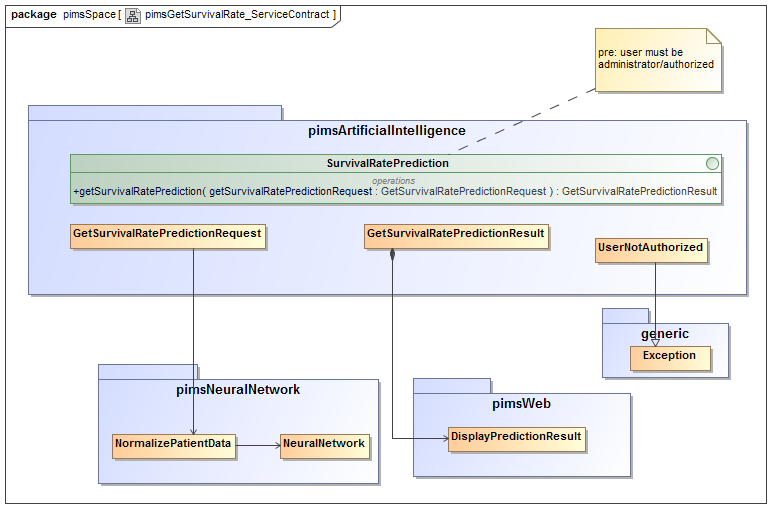
\includegraphics[width=0.8\linewidth]{./Functional_Requirements/Graphics/pimsAI/pimsGetSurvivalRate_ServiceContract}}
			\caption{Service contract for getAverageSurvivalRatePrediction}
		\end{figure}
	\end{description}
	
		\item{\textbf{getPatientChanceOfSurvival -- [priority: critical]}}
	\begin{description}
		\item{\textbf{Service Contract}} The generic service contract
		\begin{figure}[H]
			\centerline{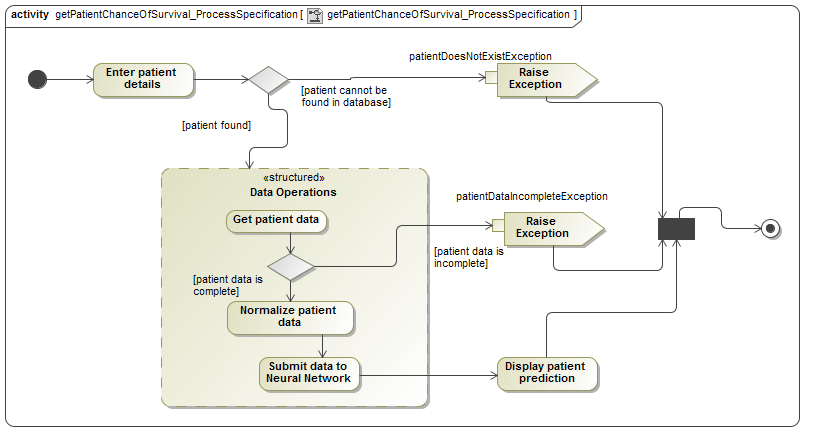
\includegraphics[width=0.9\linewidth]{./Functional_Requirements/Graphics/pimsAI/getPatientChanceOfSurvival_ProcessSpecification}}
			\caption{Process specification for Service contract for getPatientChanceOfSurvival}
		\end{figure}
	\end{description}
\end{description}

